\section{Herstellung des Rohres}
Für diesen Versuch wurde in einem CAD-Programm das Modell eines Pitot-Rohres erstellt und dieses in einem 3D-Drucker gedruckt.

\section{Messung der Fahrgeschwindigkeiten}
Um die Geschwindigkeiten des fahrenden Autos zu messen, wurde das Pitot-Rohr am Dach des Autos befestigt (Siehe \ref{rohre}), zusammen mit einem anderen, schon vorrätigen Pitot-Rohr, welches zur Messung des statischen Druckes verwendet wurde. Diese sind mit einem Feinmamnometer im Inneren des Autos verbunden worden. Mit einer ersten Kamera wurde der Stand des Manometers sowie paralel die von einem GPS-Sensor ausgegebene Geschwindigkeit aufgenommen (Siehe \ref{messung}), mit einer zweiten die Anzeige des Autotachos. Die beiden Aufnahmen wurden über die Audiospur synchronisiert, um die drei Geschwindigkeiten zu jeweils einem bestimmten Zeitpunkt auswerten zu können.

\begin{figure}
\centering
	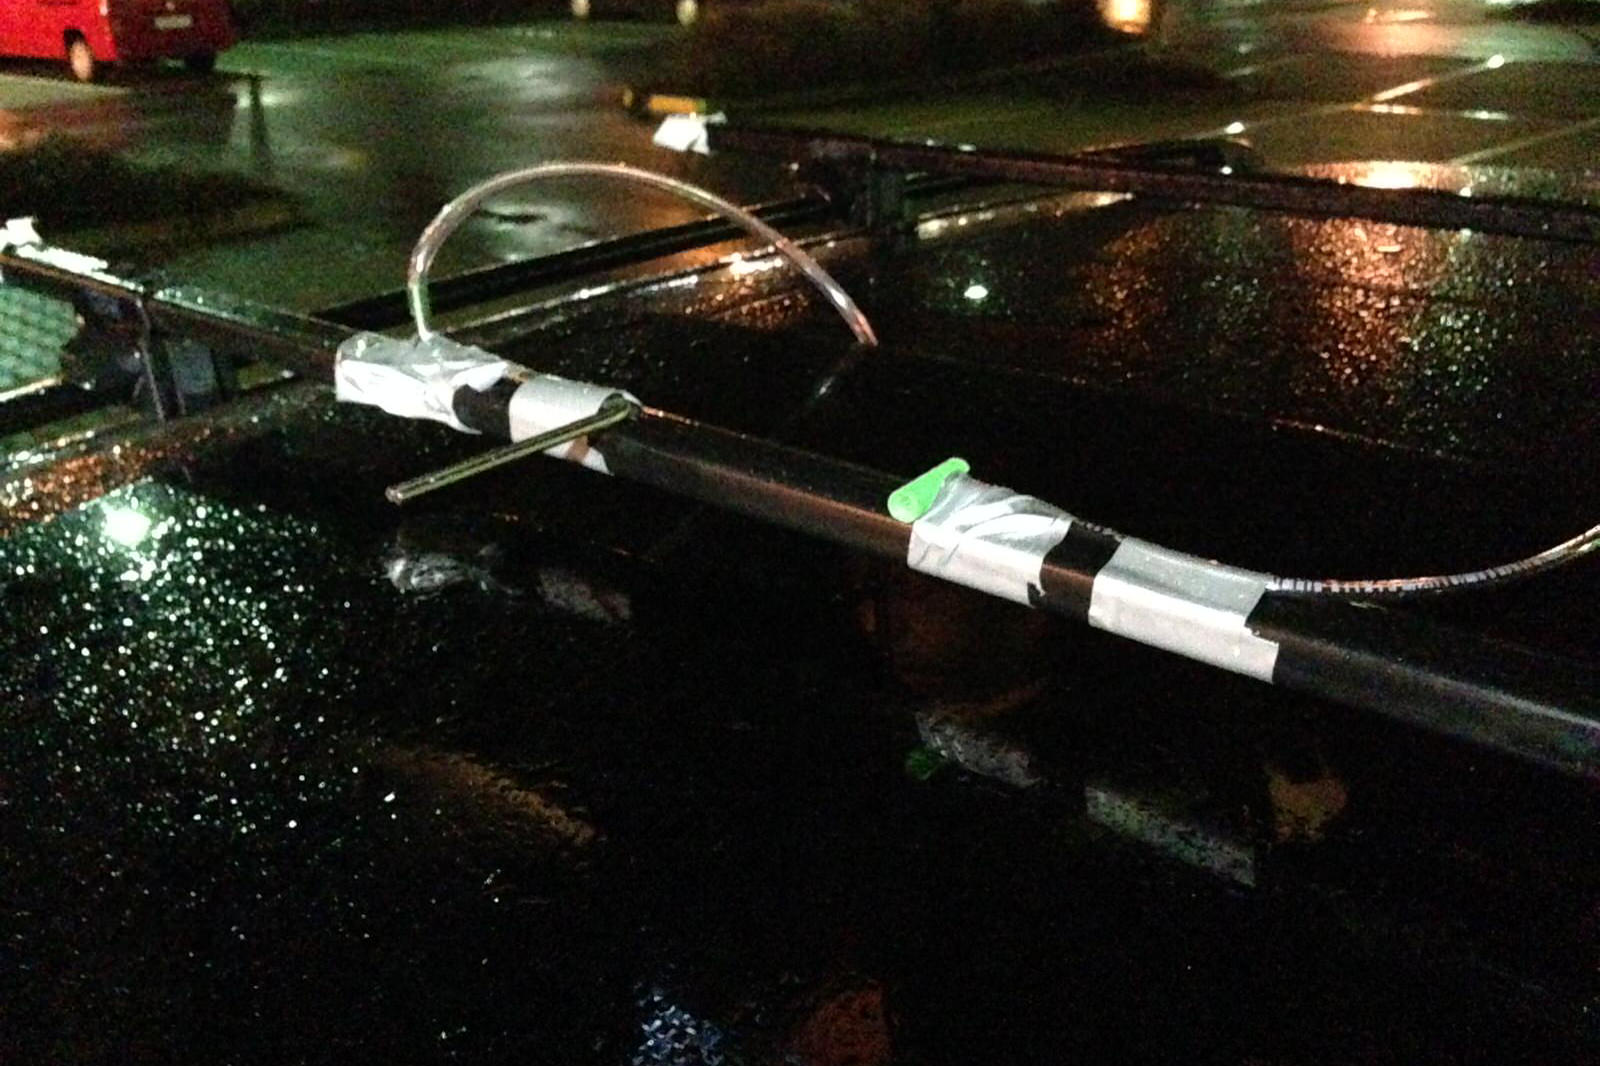
\includegraphics[width=.8\textwidth]{images/rohre.jpg}
	\caption{Bild des Versuchsaufbaus auf dem Autodach}
	\label{rohre}
\end{figure}

\begin{figure}
\centering
	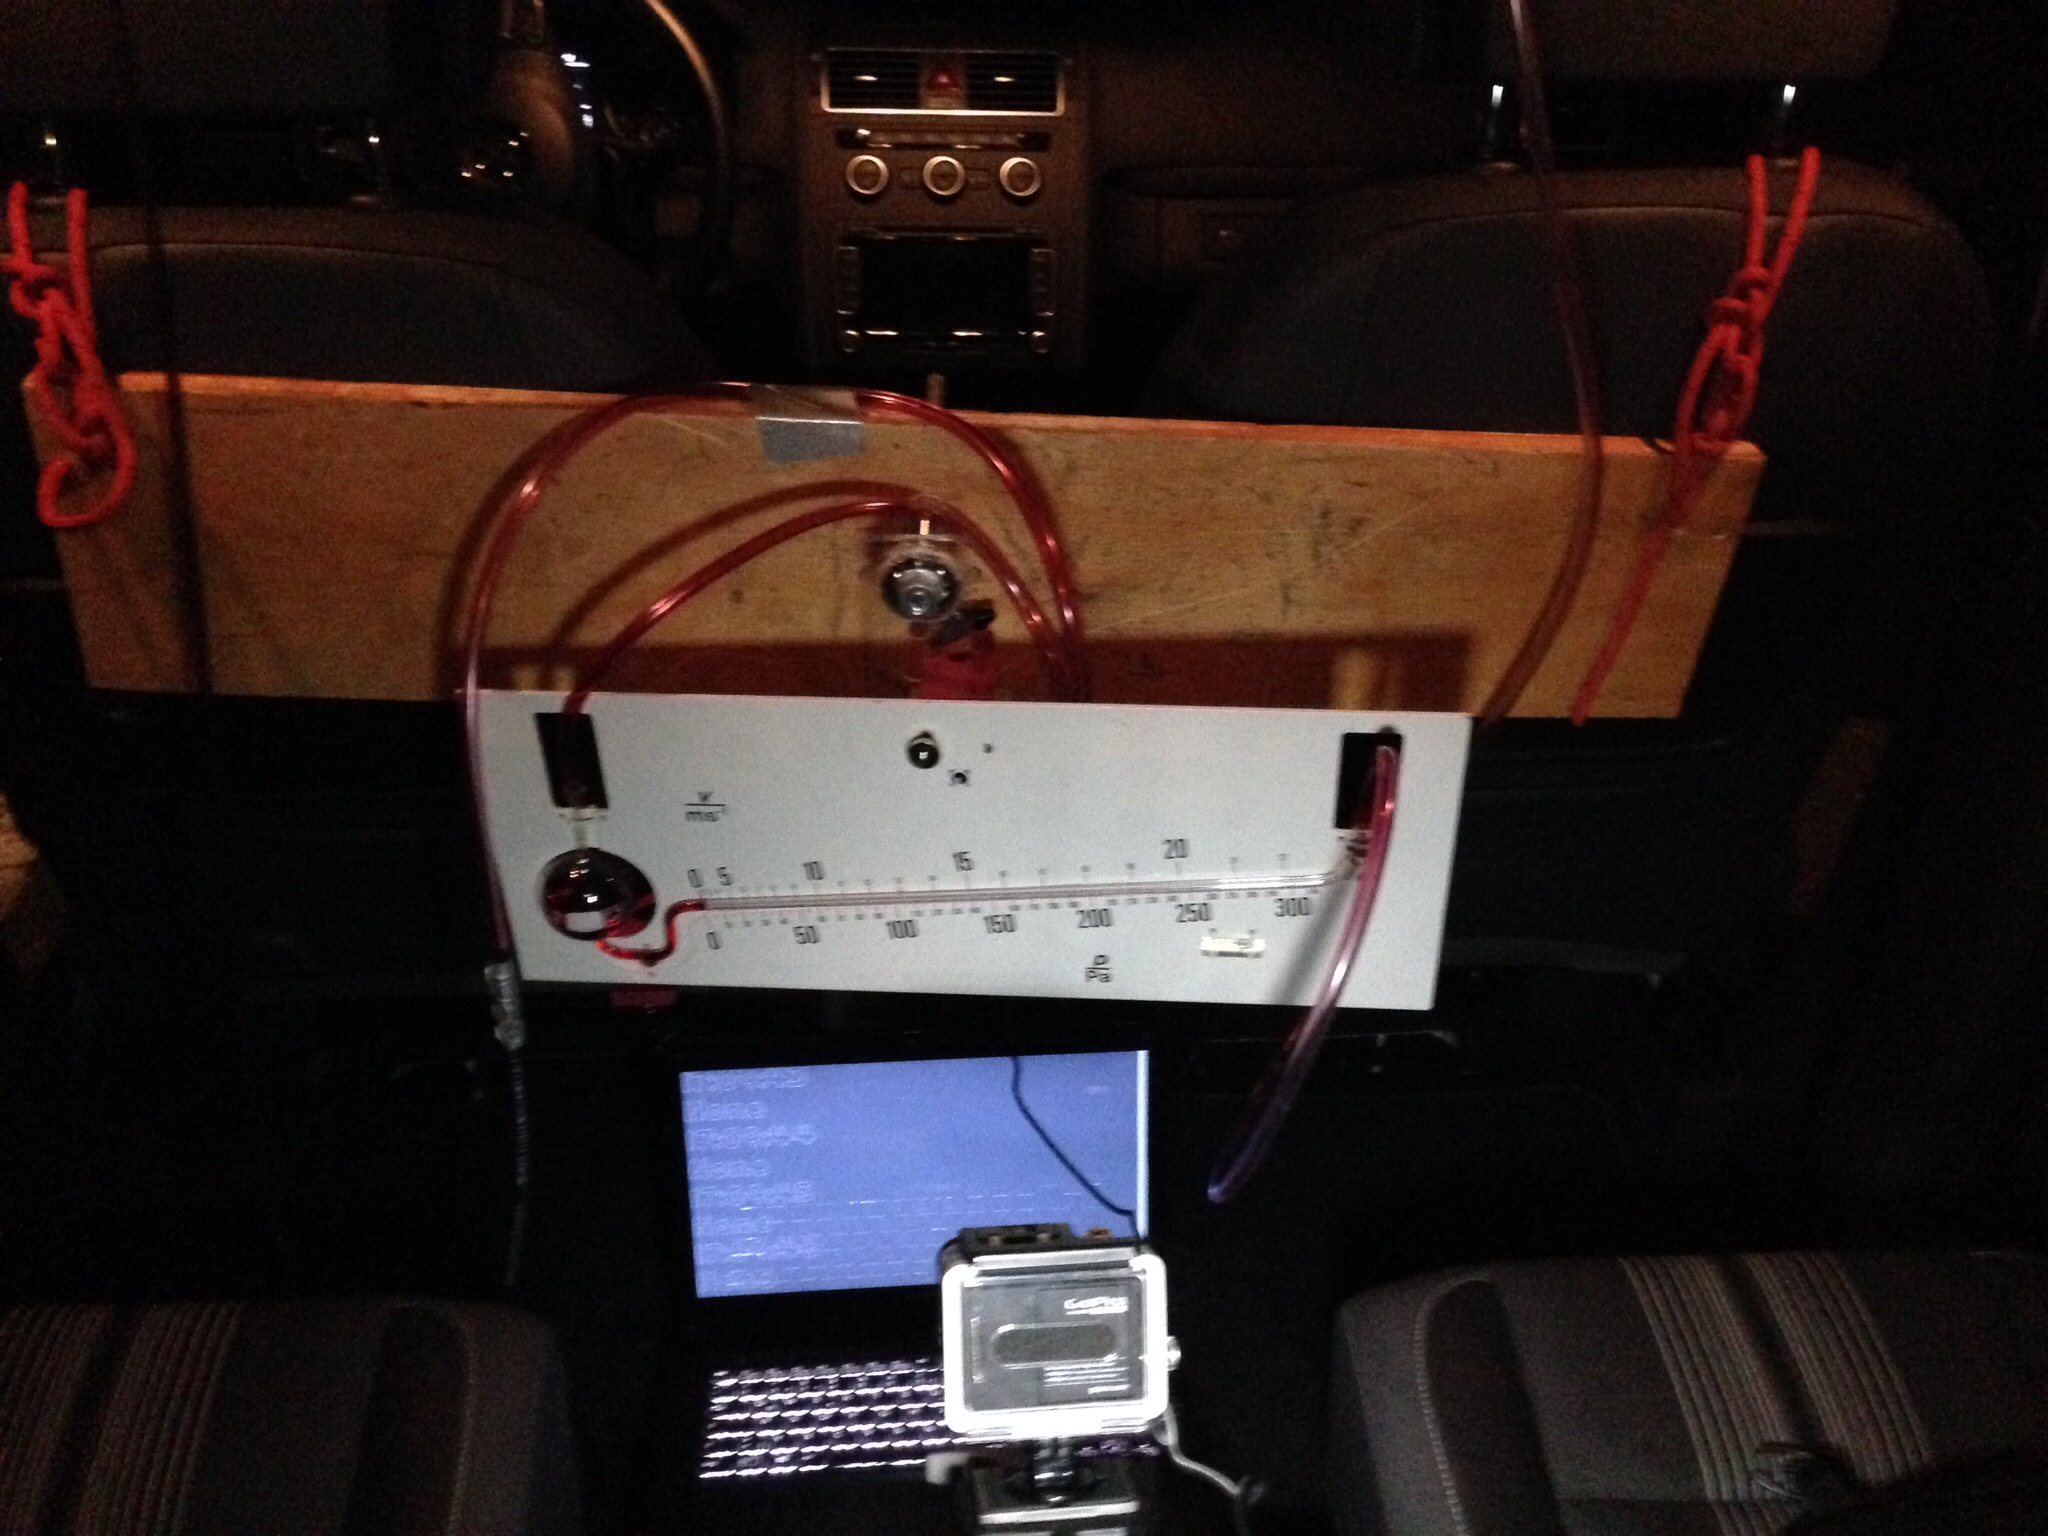
\includegraphics[width=.8\textwidth]{images/messung.jpg}
	\caption{Feinmannometer und Laptop mit GPS-Sensor}
	\label{messung}
\end{figure}

\subsection{Aufhängung des Feinmannometers}
Um mit dem Feinmannometer messen zu können, muss es genau senkrecht zum Horizont aufgerichtet werden. Dies wurde im Auto mittels einer kardanischen Aufhängung realisiert (Siehe \ref{aufhängung}): in eine frei im Auto, parallel zur Windschutzscheibe hängende Holzplatte wurde das Mannometer mittels eines Kugellagers an einer Gewindestange befestigt und diese in ein Loch in der mitte der Holzplatte eingelassen. Dies garantiert die waagrechte Ausrichting des Mannometers im Auto und gleicht leichtere Erschütterungen aus. 


\begin{figure}
\centering
	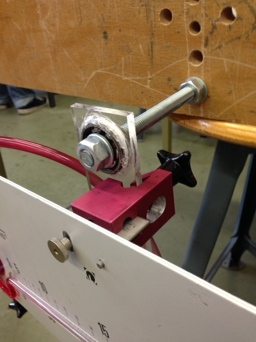
\includegraphics[width=.5\textwidth]{images/aufhaengung.JPG}
	\caption{Feinmannometer und Laptop mit GPS-Sensor}
	\label{aufhängung}
\end{figure}